\documentclass[a4,11pt]{aleph-notas}
% Se puede ver la documentación aquí: 
% https://github.com/alephsub0/LaTeX_aleph-notas

% -- Paquetes adicionales 
\usepackage{enumitem}
\usepackage{url}
\usepackage{array}
\usepackage{booktabs}
\usepackage{longtable}
\hypersetup{
    urlcolor=blue,
    linkcolor=blue,
}


% -- Datos
\institucion{Facultad de Ciencias Exactas, Naturales y Ambientale}
\carrera{Catálogo STEM}
\asignatura{Álgebra Lineal y Geometría Analítica}
\tema{Clase 02: Sistemas lineales}
\autor{Andrés Merino}
\fecha{Semestre 2025-1}

\logouno[0.14\textwidth]{Logos/logoPUCE_04_ac}
\definecolor{colortext}{HTML}{0030A1}
\definecolor{colordef}{HTML}{0030A1}
\fuente{montserrat}


\begin{document}

\encabezado

%%%%%%%%%%%%%%%%%%%%%%%%%%%%%%%%%%%%%%%%  
\section*{Resultado de Aprendizaje}  
%%%%%%%%%%%%%%%%%%%%%%%%%%%%%%%%%%%%%%%%  

%%%%%%%%%%%%%%%%%%%%%%%%%%%%%%%%%%%%%%%%  
\subsection*{RdA de la asignatura:}  
\begin{itemize}[leftmargin=*]  
    \item \textbf{RdA 1:} Comprender los conceptos básicos del Álgebra Lineal y Geometría Analítica en el campo de la Ingeniería.  
    \item \textbf{RdA 2:} Analizar los problemas relacionados al Álgebra Lineal y Geometría Analítica en el campo de la Ingeniería.  
\end{itemize}  

%%%%%%%%%%%%%%%%%%%%%%%%%%%%%%%%%%%%%%%%  
\subsection*{RdA de la actividad:}  
\begin{itemize}[leftmargin=*]  
    \item Interpretar sistemas de ecuaciones lineales desde un enfoque algebraico.  
    \item Aplicar el método de eliminación de Gauss-Jordan para resolver sistemas de ecuaciones.  
    \item Analizar la existencia y unicidad de soluciones usando el Teorema de Rouché-Frobenius.  
\end{itemize}  

%%%%%%%%%%%%%%%%%%%%%%%%%%%%%%%%%%%%%%%%  
\section*{Introducción}  
%%%%%%%%%%%%%%%%%%%%%%%%%%%%%%%%%%%%%%%%  

%%%%%%%%%%%%%%%%%%%%%%%%%%%%%%%%%%%%%%%%  
\paragraph{Pregunta inicial:}  
¿Un sistema con el mismo número de ecuaciones que incógnitas siempre tiene solución? ¿Por qué a veces no?

%%%%%%%%%%%%%%%%%%%%%%%%%%%%%%%%%%%%%%%%  
\section*{Desarrollo}  
%%%%%%%%%%%%%%%%%%%%%%%%%%%%%%%%%%%%%%%%  

%%%%%%%%%%%%%%%%%%%%%%%%%%%%%%%%%%%%%%%%  
\subsection*{Actividad 1: Resolviendo el valor de las frutas y sistemas de ecuaciones}  

La clase inicia con un reto visual que motiva el planteamiento de sistemas lineales. A través de una clase magistral, se abordan conceptos clave como operaciones por filas, eliminación de Gauss-Jordan y el Teorema de Rouché-Frobenius. Luego, se resuelven ejercicios guiados y se recomiendan recursos audiovisuales y una herramienta en línea para reforzar el aprendizaje.  

\paragraph{¿Cómo lo haremos?}  
\begin{itemize}[leftmargin=*]  
    \item \textbf{Motivación:} se presenta el reto visual con frutas y se invita a los estudiantes a plantear las ecuaciones. 
    \begin{center}
        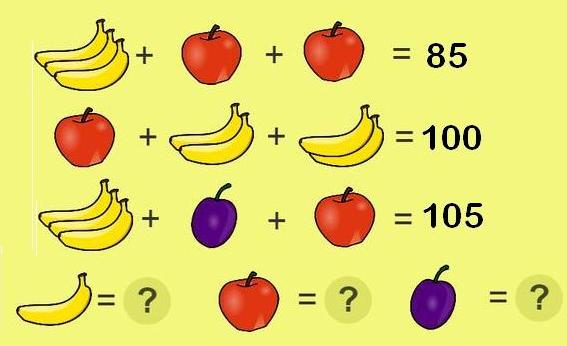
\includegraphics[width=0.5\linewidth]{2-Clases/Figuras/sistema8bien.jpg}
    \end{center}
    \item \textbf{Clase magistral:} se explican los conceptos de sistemas de ecuaciones, operaciones por filas, rango, eliminación de Gauss-Jordan, y el Teorema de Rouché-Frobenius. Se usa el resumen \href{https://fcena-puce.github.io/FCENA-PUCE/AlgLinealyGeomAnalitica-05-N0068/2-Resumenes/Resumen02.pdf}{Resumen02.pdf}.  
    \item \textbf{Resolución de ejercicios:} los estudiantes resolverán, de manera guiada, ejercicios similares a los del documento \href{https://fcena-puce.github.io/FCENA-PUCE/AlgLinealyGeomAnalitica-05-N0068/2-Ejercicios/Ejercicios02.pdf}{Ejercicios02.pdf}.  
    \item \textbf{Visualización de videos:} se recomendará el estudio con los videos:  
    \begin{itemize}
        \item \href{https://www.youtube.com/watch?v=IF7WV5VVci4}{Sistemas de dos Ecuaciones}
        \item \href{https://www.youtube.com/watch?v=dFmGzr1j6eY}{Solución de sistemas de 3x3 método de Gauss Jordan}
    \end{itemize}  
    \item \textbf{Implementación computacional:} se explica el uso de la aplicación \href{https://matrixcalc.org/es/slu.html}{Matrix Calculator} para resolver sistemas complejos.
\end{itemize}  

\paragraph{Verificación de aprendizaje:}  
\begin{itemize}[leftmargin=*]  
    \item ¿Cuándo un sistema tiene una única solución?  
    \item ¿Qué indica el rango de una matriz aumentada?  
    \item ¿En qué consiste el método de Gauss-Jordan?  
\end{itemize}  

%%%%%%%%%%%%%%%%%%%%%%%%%%%%%%%%%%%%%%%%  
\section*{Cierre}  
%%%%%%%%%%%%%%%%%%%%%%%%%%%%%%%%%%%%%%%%  

\paragraph{Tarea:}  
Resolver del libro \href{https://catalogobiblioteca.puce.edu.ec/cgi-bin/koha/opac-detail.pl?biblionumber=86083&query_desc=kw%2Cwrdl%3A%20%C3%81lgebra%20lineal%20y%20sus%20aplicaciones}{Álgebra lineal y sus aplicaciones de David C. Lay}, sección 1.2, los ejercicios: 1, 3, 7, 11 y 13.

\paragraph{Pregunta de investigación:}  
\begin{enumerate}[leftmargin=*]  
    \item ¿Qué papel juegan los sistemas lineales en el entrenamiento de modelos de inteligencia artificial?
    \item ¿Qué sucede si el sistema tiene más ecuaciones que incógnitas? ¿Y si tiene menos?  
    \item ¿Qué significa que una matriz tenga rango completo? ¿Y qué consecuencias tiene para la resolución de sistemas?
\end{enumerate}  

\paragraph{Para la próxima clase:}  
Clase invertida sobre determinantes, seguir las instrucciones disponible en \href{https://fcena-puce.github.io/FCENA-PUCE/AlgLinealyGeomAnalitica-05-N0068/2-ClaseInvertida/00Est-Determinantes.pdf}{01Est-Determinantes.pdf}.  


\end{document} 